\documentclass[ai,article,submit,moreauthors]{Definitions/mdpi}
\firstpage{1}
\makeatletter
\setcounter{page}{\@firstpage}
\makeatother
\pubvolume{1}
\issuenum{1}
\articlenumber{0}
\pubyear{2026}
\copyrightyear{2026}
\datereceived{ }
\daterevised{ }
\dateaccepted{ }
\datepublished{ }
\usepackage{longtable,placeins}
\setlength{\emergencystretch}{2em}
\setlength{\headheight}{20pt}
% No article DOI has been assigned; suppress the template-generated dummy link.
\AtBeginDocument{\fancyfoot[R]{}}
\makeatletter
\apptocmd{\ps@plain}{\fancyfoot[R]{}}{}{}
\makeatother
\Title{Stream Reduction in Multi-Stream Graph Convolutional Networks: A Non-Inferiority Study for Skeleton-Based Action Recognition}
% Names, order, correspondence and affiliations transcribed from the supplied author document.
\newcommand{\orcidauthorA}{0009-0005-8440-9106}
\newcommand{\orcidauthorB}{0000-0003-2331-6326}
\newcommand{\orcidauthorC}{0000-0002-3164-3688}
\newcommand{\orcidauthorD}{0000-0002-1245-8313}
\newcommand{\orcidauthorE}{0000-0002-1353-2677}
\newcommand{\orcidauthorF}{0000-0003-0698-666X}
\Author{Aida Issembayeva $^{1}$\orcidA{}, Oleksandr Kuznetsov $^{2,3,4,}$*\orcidB{}, Anargul Shaushenova $^{1,}$*\orcidC{}, Ardak Nurpeisova $^{1}$\orcidD{}, Lyazzat Zhumaliyeva $^{5}$\orcidE{} and Maral Ongarbayeva $^{6}$\orcidF{}}
\AuthorNames{Aida Issembayeva, Oleksandr Kuznetsov, Anargul Shaushenova, Ardak Nurpeisova, Lyazzat Zhumaliyeva and Maral Ongarbayeva}
\address{%
$^{1}$ \quad Department of Information Systems, Faculty of Computer Systems and Professional Education, Saken Seifullin Kazakh Agrotechnical University, Astana 010000, Kazakhstan; a.issembayeva@kazatu.edu.kz (A.I.); a.nurpeisova@kazatu.edu.kz (A.N.)\\
$^{2}$ \quad Department of Theoretical and Applied Sciences, eCampus University, Via Isimbardi 10, 22060 Novedrate (CO), Italy\\
$^{3}$ \quad SMARTEST Research Center, eCampus University, Via Isimbardi 10, 22060 Novedrate (CO), Italy\\
$^{4}$ \quad Department of Intelligent Software Systems and Technologies, School of Computer Science and Artificial Intelligence, V. N. Karazin Kharkiv National University, 4 Svobody Sq., 61022 Kharkiv, Ukraine\\
$^{5}$ \quad Department of Physics, Mathematics and Computer Science, Astana International University, Astana 010000, Kazakhstan; lyazzat\_zhumalieva@aiu.edu.kz\\
$^{6}$ \quad Department of Information and Communication Technologies, Faculty of Natural Sciences, International Taraz University Named After Sherkhan Murtaza, Taraz 080000, Kazakhstan; ongarbaeva@htu.kz}
\corres{Correspondence: oleksandr.kuznetsov@uniecampus.it (O.K.); a.shaushenova@kazatu.edu.kz (A.S.)}

\abstract{Multi-stream graph convolutional networks improve skeleton action recognition by combining representations, but each branch adds inference cost. We evaluate the marginal cost and quality contribution of one stream using a paired non-inferiority protocol on NTU RGB+D 120. A temporal reduction first decreased logical skeleton reads by 53.52\%, but lost 3.191 percentage points of accuracy and provided no fresh-mapping latency saving. A three-stream configuration then omitted bone motion while retaining 64 temporal positions. Earlier RTX 4090 measurements at batch size one showed 24.30--24.94\% lower latency. After development confirmation, the fixed pair was trained on 54,468 examples and evaluated on 59,477 cross-setup test examples. Overall accuracy was 89.1050\% for four streams and 89.0277\% for three streams; paired setup-bootstrap lower bounds exceeded all three prespecified non-inferiority margins. Stream removal introduced 605 errors and corrected 559, while predicted labels changed for 1,778 examples. Thus, a net loss of 46 correct decisions concealed broader redistribution. Recall decreased for 61 of 120 actions. These findings support assessing a branch by its contribution to the complete system, measured cost, and explicit quality tolerances. They do not imply preservation of every action. Final-checkpoint latency was not remeasured.}
\keyword{graph neural networks; skeleton-based action recognition; efficient inference; multi-stream fusion; non-inferiority; CTR-GCN}
\begin{document}
\section{Introduction}
Skeleton-based action recognition represents a person's movement as a sequence of articulated joint positions. This compact description separates much of the motion information from appearance and is useful when the task concerns how a person moves rather than what the scene looks like. Its computational cost nevertheless depends on more than the size of the input. A multi-stream system may process several transformations of the same skeleton sequence through separate networks. Each branch offers a different view of the action, but also adds a forward pass to the recognition pipeline.

For deployment, the relevant question is whether the contribution of an additional branch justifies its measured cost. A small increase in benchmark accuracy can be useful, yet a system with a tight response-time budget may prefer a simpler operating point if the quality loss is bounded. Conversely, reducing the number of input observations can be ineffective when neural inference, rather than input access, dominates execution. Both possibilities call for an evaluation that pairs recognition quality with a clearly defined timing boundary.

We study the marginal value of skeleton representations in a four-stream CTR-GCN system on NTU RGB+D 120 under the cross-setup protocol. Two interventions act on different parts of the computation: reading fewer source frames and omitting the bone-motion stream while retaining 64 temporal positions. For the stream comparison, the retained models and their relative fusion weights are shared between systems. This isolates the contribution of the omitted branch within the selected ensemble.

The study asks three questions. Does reducing source-frame access produce useful pipeline acceleration? Can a complete stream be removed while meeting explicit tolerances for aggregate quality? How does this simplification redistribute decisions across actions and acquisition setups? We distinguish exploratory selection, a development follow-up under a new training seed schedule, hardware timing, and a final fixed test comparison.

The contribution is a controlled assessment of where computation can be removed from a multi-stream graph-convolution system. We combine measured latency with prespecified tolerances for overall accuracy, accuracy on the additional NTU120 actions, and macro-F1. The comparison distinguishes an ineffective temporal configuration from a useful reduction in stream count. Paired decision analysis then shows why a small aggregate loss does not imply that the systems make the same errors. The resulting protocol and saved-output analysis provide a reproducible way to assess this operating point; a new graph-convolution architecture or statistical estimator is not proposed.

\section{Related Work}
\subsection{Graph models and complementary skeleton representations}
Spatial temporal graph convolutional networks model body joints and their temporal connections directly, avoiding a hand-designed sequence descriptor \cite{yan2018stgcn}. Adaptive graph approaches extend this representation by learning graph structure; the two-stream adaptive GCN also uses joint and bone information as complementary inputs \cite{shi2019twostream}. MS-G3D develops multi-scale spatial aggregation and spatial--temporal graph modeling \cite{liu2020msg3d}. CTR-GCN refines topology on a channel-wise basis \cite{chen2021ctrgcn}. More recently, BlockGCN has revisited topology and channel grouping within graph convolution \cite{zhou2024blockgcn}. These advances provide the architectural background for the reference used here.

Our four inputs are transformations of the same measured skeleton sequence, not four independently acquired sensor modalities. Joint positions, bone vectors, and their temporal differences emphasize different properties of the motion. Four-stream joint, bone, joint-motion and bone-motion fusion is already established in MS-AAGCN \cite{shi2020multistream}. Their complementarity motivates multi-stream fusion, but does not imply that every stream is equally useful for every action. A paired comparison with shared retained checkpoints isolates the effect of excluding a stream from a particular trained ensemble.

\subsection{Efficiency and the scope of the present comparison}
Efficient skeleton recognition has been pursued through architectural changes as well as adaptive computation. Shift-GCN uses shift operations to reduce the cost of graph-convolution processing \cite{cheng2020shiftgcn}. EfficientGCN combines multiple inputs within an efficient network and uses separable operations and compound scaling \cite{song2022efficientgcn}. AdaSGN adapts the graph choice to reduce computation \cite{shi2021adasgn}, whereas HPI-GCN studies re-parameterization and over-parameterization for inference \cite{wang2025hpi}. These methods address different parts of the recognition problem and should not be ranked using latencies obtained on different devices or with different measurement boundaries.

Architecture-level comparisons do not directly determine the contribution of one branch within a particular trained ensemble. The present work holds the reference architecture and shared models fixed within each stream-comparison pair. Its scope is consequently narrower than a benchmark of efficient architectures: it measures the marginal cost and quality contribution of one branch, after examining a temporal alternative. The added evidence is the separation of development from final testing, the use of predetermined loss tolerances, and a paired analysis that preserves setup-level clustering. Passing the decision rule means that the observed system meets those tolerances under the stated resampling assumptions; it does not prove that the two systems are identical or that the simplification is optimal.
\section{Materials and Methods}

\subsection{Reference Model and System Comparison}

Each sample is represented by three-dimensional coordinates for 25 joints and at most two people. Let $x_{t,v}$ denote the coordinates of joint $v$ at output time $t$, and let $p(v)$ be its parent in the fixed NTU skeleton graph. Bone vectors are $b_{t,v}=x_{t,v}-x_{t,p(v)}$. Joint motion and bone motion are first temporal differences, $x_{t+1,v}-x_{t,v}$ and $b_{t+1,v}-b_{t,v}$; their final temporal positions are set to zero. All four inputs therefore derive from the same skeleton observations.

The reference has ten graph--temporal blocks, with 64 channels in blocks one to four, 128 in blocks five to seven, and 256 in blocks eight to ten. Temporal stride two is used in blocks five and eight. Adaptive topology is enabled. Global averaging over the remaining temporal, joint, and person dimensions precedes a 120-class linear layer. Dropout is disabled. We use this architecturally matched implementation of CTR-GCN \cite{chen2021ctrgcn} consistently throughout the selected comparison; the training recipe and data processing define a reference experiment rather than a reproduction claim for the original paper's reported score.

The Full-4 reference contains joint, bone, joint-motion, and bone-motion
streams. For sample $i$, let $z_{is}\in\mathbb{R}^{120}$ denote the logits
from stream $s$. The two systems are
\begin{align}
 z_i^{(4)} &=0.3z_{i0}+0.3z_{i1}+0.2z_{i2}+0.2z_{i3},\\
 z_i^{(3)} &=0.375z_{i0}+0.375z_{i1}+0.25z_{i2}.
\end{align}
Stream-3 excludes bone motion. The retained three checkpoints are identical
between the two systems within each comparison. No fusion weights or
temperatures are fitted. The frozen implementation combines logits in
float32 with the same operation order for all samples and applies an argmax
over all 120 classes.

The temporal development study used base seed 271828 and separately trained
the four streams for $K\in\{8,16,32,64\}$. K64 used crop-and-resize, whereas
K8, K16, and K32 used exact uniform sampling. K32 was the prespecified primary
temporal configuration; its unsuccessful result was retained. Stream-3 was selected
subsequently by exploratory analysis of saved development predictions. Its
quality protocol was then frozen before new training with base seed 161803.
Finally, the selected Full-4/Stream-3 pair was fixed before the official XSet
evaluation. This chronology separates the exploratory selection from the
later checks; it does not recast the entire study as prospectively selected.

\subsection{Dataset Partitions and Prior Exposure}

The study uses the existing processed skeleton data from NTU RGB+D 120 under
the XSet protocol \cite{shahroudy2016ntu60,liu2019ntu120}. The retained
development training partition contains 38,670 samples from 12 setups.
Its three held-out folds are $(4,12,18,26)$, $(6,14,22,28)$, and
$(8,16,24,32)$. Each sample receives exactly one out-of-fold prediction from
a model that was not trained on its setup. The former validation partition
contains 15,798 samples from setups $(2,10,20,30)$. It and the XSet test
were excluded from the temporal and new-seed out-of-fold experiments.

For final training, the official training population contains 54,468 retained
samples: the 38,670 base-training samples followed by the 15,798 former
validation samples. The latter are used only for training in this final stage.
No metric is computed on them for checkpoint or parameter selection. The
final XSet test contains 59,477 retained samples from the 16 odd-numbered
setups. Canonical manifests establish the sample order, labels, and setup
membership. Their sample IDs are unique and disjoint across the original
train, validation, and test partitions. Existing preprocessing is reused.

NTU RGB+D 120 extends NTU RGB+D with additional actions \cite{ntuofficial}.
Earlier stages of the project used NTU60, so A1--A60 cannot be presented as
independent of the complete research history. A61--A120 provides the strongest
held-out interpretation for the final test examples within the documented
history. These actions are represented in training; the endpoint is not a
zero-shot evaluation. It contains 29,375 test samples in setups
19, 21, 23, 25, 27, 29, and 31. The remaining 30,102 samples belong to
A1--A60. All of these evaluations remain within NTU RGB+D 120.

\subsection{Training and Temporal Representation}

The new-seed development follow-up comprises four streams in each of three
folds. Its job seed is $161803+1000(f-1)+10s$, where $f$ is the one-based
fold index and $s$ is the zero-based stream index. Final training instead
uses four full-training models with seeds 161803, 161813, 161823, and 161833.
The full-training checkpoints are newly fitted models, not an ensemble of
the earlier fold checkpoints.

All these trainings use 65 epochs of SGD with batch size 64, initial learning
rate 0.1, momentum 0.9, Nesterov acceleration, and weight decay
$4\times10^{-4}$. The learning rate has five warm-up epochs and reductions
by a factor of 0.1 at epochs 35 and 55. Label smoothing and automatic mixed
precision are disabled. The final epoch is retained without validation
monitoring. Deterministic algorithms are requested in warning mode;
bitwise agreement across arbitrary hardware and software environments is
not claimed.

K64 uses 64 output frames with crop-and-resize temporal interpolation.
Training uses a random crop proportion in $[0.5,1.0]$ and rotation augmentation
with independent angles sampled uniformly from $[-0.3,0.3]$ radians around each axis. Evaluation uses a centered crop with
proportion 0.95 and no rotation. The sparse adapter reads the interpolation
supports from the existing skeleton store. In final training, base-training
samples use that store, while former-validation samples use the existing
processed NPZ files with the same support and interpolation operations.
Final test samples use the NPZ adapter. The preflight records exact tensor
and temporal-index parity on 432 prescribed base-training cases; no test
tensor is used for that parity check.

\subsection{Final Evaluation and Numerical Reproduction}
All four final models were trained before evaluating the selected system pair. Their identities, the data partitions, the fusion rules, and the analysis protocol were fixed before the final test evaluation. One saved prediction matrix per stream supplies both systems. Stream-3 reuses the retained three streams; no second forward pass or separate checkpoint selection is involved.

The analysis checks sample identifiers, class labels, setup labels, and temporal-position metadata across the four prediction files. It then reconstructs both fused outputs and all reported endpoints. A separate implementation uses per-setup class counts to reproduce the bootstrap, providing a check against the original confusion-matrix implementation. This verifies the saved-output calculations without rerunning training or inference. Supplementary Materials describe the evidence coverage and the distinction between reproducing an analysis and reproducing model training.

\subsection{Quality Criteria and Paired Bootstrap}

The three quality endpoints are overall Top-1, Top-1 on A61--A120, and
macro-F1 over all 120 classes. Let $\widehat\Delta_j$ be Stream-3 minus
Full-4 for endpoint $j$. The fixed non-inferiority margins on the unit scale
are $m=(-0.010,-0.015,-0.015)$. These tolerances define the study's decision
rule; they are not universal tolerances for every application or action. Non-inferiority is assessed against an explicitly chosen margin rather than inferred from a nonsignificant difference \cite{walker2011noninferiority}. The margins here are operational study choices; they were not derived from a user study or a domain-specific cost model.

The bootstrap \cite{efron1979bootstrap} approximates sampling variation by resampling acquisition setups as clusters, while preserving the pairing of the two systems. Resampling clusters rather than individual sequences reflects the grouping imposed by the XSet evaluation, although it cannot remove all dependence between subjects recorded in different setups. A paired setup-cluster bootstrap resamples setups with replacement and
includes all samples from each selected setup with the selected multiplicity.
Both systems use the same replicate. Preserving dependence and pairing is central to interpretable resampling for comparative measurements \cite{bakshy2013dependentbootstrap}. Accuracy is computed over the resulting
sample union, not as an equally weighted average of setup accuracies.
Macro-F1 is recalculated within each replicate as
\begin{equation}
 F_{\mathrm{macro}}=\frac{1}{120}\sum_{c=1}^{120}
 \frac{2\,TP_c}{N_c+\widehat N_c},
\end{equation}
where $N_c$ and $\widehat N_c$ are true and predicted class counts. A term
with zero denominator is set to zero. The class set is not reduced when a
bootstrap draw lacks support for an action.

The development follow-up resamples its 12 setups. The final protocol uses
10,000 replicates of the 16 test setups. A pool of 20,000 index rows is
frozen with seed 223607. Before training, canonical test metadata select
the first 10,000 rows with nonzero A61--A120 support; no prediction is used
in this selection. The actual selected pool required no rejected rows.
The saved index array and its raw little-endian int64 hash are verified
independently during the audit.

With $\alpha_j=0.05/3$, the one-sided centered-basic lower bound is
\begin{equation}
 L_j=2\widehat\Delta_j-
 Q_{1-\alpha_j}\!\left(\widehat\Delta_j^{\,*}\right),
\end{equation}
using the higher empirical quantile. Non-inferiority is established under the study rule only if
$L_j>m_j$ for all three endpoints. The frozen Bonferroni allocation is
retained throughout. The corresponding resampling p-value is
\begin{equation}
 p_j=\frac{1+\sum_{b=1}^{B}
 \mathbf{1}\{\widehat\Delta_{jb}^{*}-\widehat\Delta_j
 \geq\widehat\Delta_j-m_j\}}{B+1},\qquad B=10000,
\end{equation}
with adjusted value $\min(1,3p_j)$. These are approximate cluster-bootstrap
inferences conditional on the fitted models. Setup and class summaries are
descriptive and cannot alter the criteria, margins, candidate, or checkpoint.

\subsection{Latency Measurement}

The Stream-3 latency experiment used the existing seed-271828 checkpoints,
an RTX 4090, and batch size one. Eighteen paired traces cover three folds,
two mapping regimes, and three process repetitions. Each trace has 400
samples, with 100 from each held-out setup, after 30 warm-up samples per
system. For each sample and system, the median of the three process repetitions is computed first; reported latency is then the mean of those per-sample medians over 1,200 samples in each regime. Its separate setup-cluster procedure resamples these aggregated paired observations and adjusts for the two latency
endpoints. The resulting bounds do not include the full variability between processes or devices. The prespecified requirement is a one-sided lower bound greater
than 20\% saving in both regimes.

Timing begins at dataset sample access and includes skeleton preparation,
modality construction, host-to-device transfer, sequential network forwards,
weighted fusion, argmax, and CUDA synchronization. Model loading and
dataset-object construction are excluded. Warm reuse retains a dataset
object. Fresh mapping constructs a new dataset object before timing starts;
it does not guarantee a cold operating-system page cache. The latency
and quality stages use different seed-specific checkpoints with the same
architecture and stream composition. The final models were not benchmarked
again. Temporal and stream-reduction campaigns retain their own paired
Full-4 references; their absolute timings are not pooled.

\subsection{Research Workflow and AI Assistance}
ChatGPT (OpenAI) was used to assist with software development, analysis scripts, literature organization, interpretation, and manuscript drafting and revision. Numerical results in this article originate from the recorded experiments and deterministic analysis of saved outputs; they were not generated as illustrative data. The numerical reproduction checks described above were executed on the supplied evidence. The authors retain responsibility for the scientific claims, the supporting code and evidence, and the final text.

\section{Results}

\subsection{Temporal Reduction Did Not Meet the Efficiency Criterion}

The primary K32 configuration reduced mean logical skeleton reads by 53.52\%,
but decreased overall Top-1 by 3.191 percentage points and produced
$-0.100\%$ fresh-mapping latency saving (Table~\ref{tab:temporal}).
K16 and K8 further reduced reads while losing more accuracy; their measured
savings remained below one percent. The lower-$K$ points remain historical
secondary configurations and do not redefine the primary K32 result.
Logical source access is a property of the skeleton store, not a measurement
of RGB acquisition or sensor energy.

\begin{table}[H]
\centering\small\setlength{\tabcolsep}{3pt}
\caption{Temporal development results, seed 271828. Each variant was trained
separately. Latency saving uses the paired reference from that campaign.}
\label{tab:temporal}
\begin{tabular}{lrrrr}
\toprule
Variant & All Top-1 (\%) & A61--A120 (\%) & Read reduction (\%) & Saving (\%)\\
\midrule
K64 resize & 83.659 & 81.191 & 0.00 & 0.000\\
K32 exact & 80.468 & 76.773 & 53.52 & -0.100\\
K16 exact & 78.172 & 74.744 & 76.62 & 0.036\\
K8 exact & 75.115 & 72.966 & 88.31 & 0.477\\
\bottomrule
\end{tabular}
\end{table}

The saved fresh-mapping profile records 56.177438 ms for the reference and
55.2887745 ms for K32 inference alone. If this inference time stays fixed
and all remaining overhead is idealized as zero, the saving ceiling is
\begin{equation}
 1-\frac{55.2887745}{56.177438}=1.5819\%.
\end{equation}
The analogous warm-reuse value is 0.8849\%. These are conditional diagnostics
from aggregated timings, not confidence bounds or hardware-independent
limits. K64 and K32 also differ in temporal resampling: crop-and-resize versus exact uniform sampling. Their accuracy difference therefore cannot be attributed to frame count alone. Motion inputs are consecutive sampled-frame differences without normalization by elapsed time, so changing the sampling pattern also changes those features. Separately aggregated stage timings need not sum exactly to an
aggregated total.

\subsection{Measured Latency of the Three-Stream System}

Warm-reuse latency fell from 65.2755 to 48.9959 ms and fresh-mapping latency
from 68.5097 to 51.8634 ms (Table~\ref{tab:latency}). The savings were
24.9399\% and 24.2977\%, respectively. Both lower bounds exceeded 20\%.
Figure~\ref{fig:interventions} presents the temporal quality cost and the
separately measured stream-reduction latency benefit.

\begin{table}[H]
\centering\small\setlength{\tabcolsep}{3pt}
\caption{Earlier Stream-3 latency measurements: RTX 4090, batch one,
seed-271828 checkpoints. Final checkpoint latency was not remeasured.}
\label{tab:latency}
\begin{tabular}{lrrrr}
\toprule
Regime & Full-4 (ms) & Stream-3 (ms) & Saving (\%) & Lower bound (\%)\\
\midrule
Warm reuse & 65.2755 & 48.9959 & 24.9399 & 24.8819\\
Fresh mapping & 68.5097 & 51.8634 & 24.2977 & 24.2223\\
\bottomrule
\end{tabular}
\end{table}

\begin{figure}[H]
\centering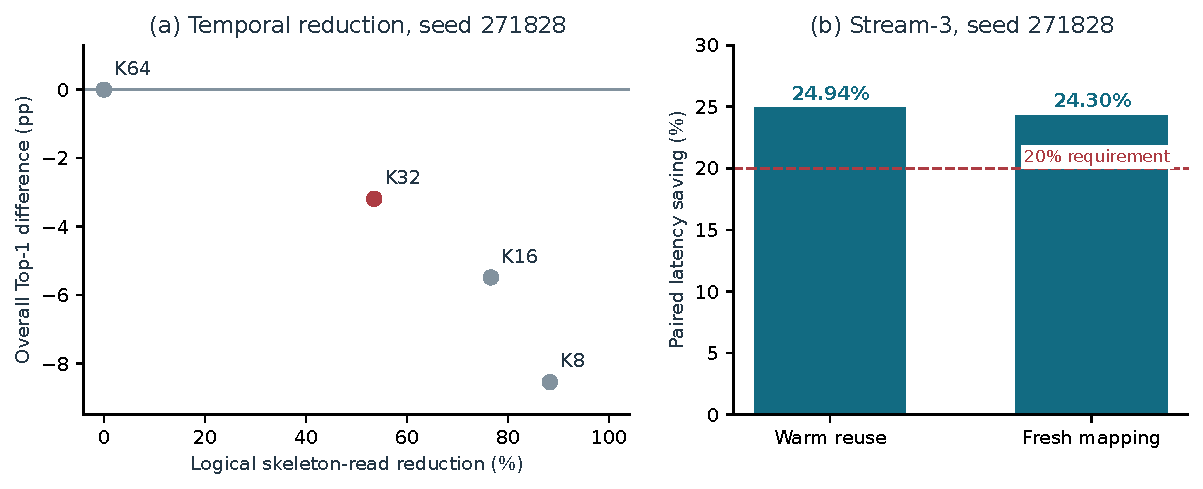
\includegraphics[width=\linewidth]{figures/TEMPORAL_AND_STREAM_EVIDENCE.pdf}
\caption{Historical interventions. (a) Greater logical-read reduction was
associated with larger accuracy loss in the temporal configurations.
(b) Stream-3 met both latency requirements in its separate measurement campaign.
Panel (a) does not imply that read reduction is a latency measurement.}
\label{fig:interventions}
\end{figure}

\subsection{Development Confirmation under a New Seed Schedule}

The frozen follow-up met all three non-inferiority criteria (Table~\ref{tab:development}).
Full-4 correctly classified 32,393 of 38,670 samples and Stream-3 classified
32,259. There were 600 correct-to-error transitions and 466 error-to-correct
transitions, giving 134 additional errors. Fold differences in overall Top-1
were $-0.024$, $-0.279$, and $-0.707$ percentage points. These results
support repeatability under the new training seed schedule on the same
development samples and fold plan. They are not an independent-dataset test.

\begin{table}[H]
\centering\small\setlength{\tabcolsep}{3pt}
\caption{Development confirmation, base seed 161803. Metrics are percentages;
differences, lower bounds, and margins are percentage points.}
\label{tab:development}
\begin{tabular}{lrrrrr}
\toprule
Endpoint & Full-4 & Stream-3 & Difference & Lower bound & Margin\\
\midrule
Overall Top-1 & 83.768 & 83.421 & -0.347 & -0.661 & -1.000\\
A61--A120 Top-1 & 81.722 & 81.632 & -0.089 & -0.546 & -1.500\\
Macro-F1 & 83.791 & 83.456 & -0.335 & -0.601 & -1.500\\
\bottomrule
\end{tabular}
\end{table}

\subsection{Final Cross-Setup Evaluation}

The final paired comparison met all three prespecified quality
gates (Table~\ref{tab:final}; Figure~\ref{fig:gate}). Overall Top-1 was
89.1050\% for Full-4 and 89.0277\% for Stream-3. The difference was
$-0.0773$ percentage points, with a lower bound of $-0.2041$ percentage
points against the $-1.0$ margin. For A61--A120, the difference was
$-0.2009$ percentage points and its lower bound was $-0.3693$, against
the $-1.5$ margin. Macro-F1 decreased by 0.0826 percentage points, with a
lower bound of $-0.2647$, also above $-1.5$.

\begin{table}[H]
\centering\small\setlength{\tabcolsep}{3pt}\setlength{\tabcolsep}{3pt}
\caption{Final paired XSet comparison from the four saved stream
logit files. Metrics are percentages; differences, lower bounds, and margins
are percentage points. All three criteria are met.}
\label{tab:final}
\begin{tabular}{lrrrrr}
\toprule
Endpoint & Full-4 & Stream-3 & Difference & Lower bound & Margin \\
\midrule
Overall Top-1 & 89.1050 & 89.0277 & -0.0773 & -0.2041 & -1.0000 \\
A61--A120 Top-1 & 87.0672 & 86.8664 & -0.2009 & -0.3693 & -1.5000 \\
Macro-F1, all 120 & 89.1059 & 89.0233 & -0.0826 & -0.2647 & -1.5000 \\
\bottomrule
\end{tabular}

\end{table}

All three adjusted resampling p-values were 0.0002999700. The underlying
value $1/10001$ is the minimum permitted by the implemented finite-resample
formula; it is not a claim of zero probability. The decision follows the
frozen lower-bound rule.

\begin{figure}[H]
\centering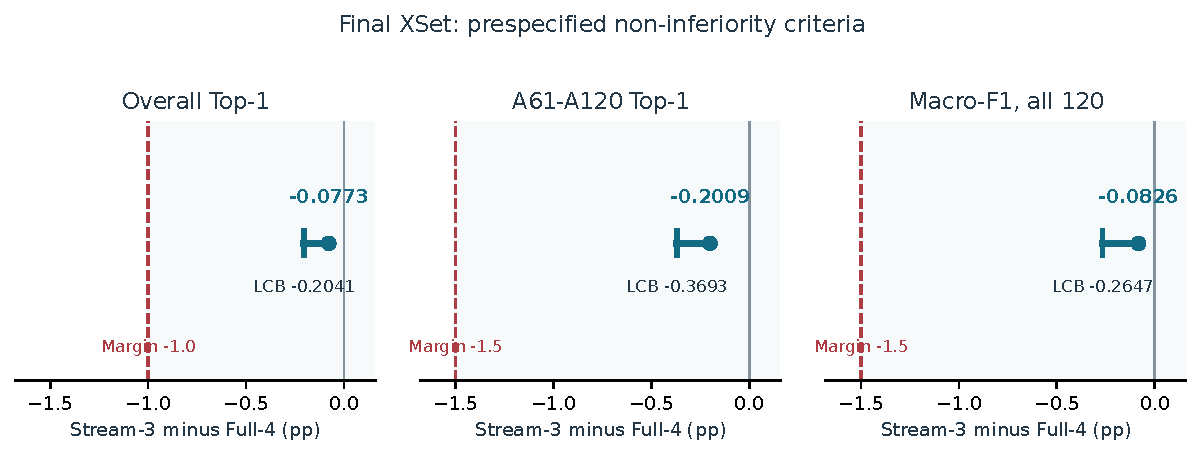
\includegraphics[width=\linewidth]{figures/FINAL_NONINFERIORITY.pdf}
\caption{Final quality criteria. Each segment connects a one-sided lower
bound to the point estimate; it is not a two-sided confidence interval.
Dashed lines show the unchanged margins.}
\label{fig:gate}
\end{figure}

Full-4 produced 52,997 correct decisions and Stream-3 produced 52,951.
Stream removal changed 605 correct decisions into errors and corrected
559 reference errors. The net cost was 46 additional errors, or 0.7734 per
1,000 test samples. For A61--A120, the counts were 25,576 and 25,517 among
29,375 samples: 59 fewer correct decisions. For A1--A60, the counts were
27,421 and 27,434 among 30,102 samples: 13 more correct decisions.
These group counts describe the distribution of the aggregate effect and do not define another selection or testing stage.

\begin{table}[H]
\centering\small
\caption{Paired correctness of the two fixed systems on all 59,477 test examples. Rows refer to Full-4 and columns to Stream-3. The off-diagonal entries distinguish introduced from corrected errors.}
\label{tab:paired}
\begin{tabular}{lrrr}
\toprule
Full-4 outcome & Stream-3 correct & Stream-3 incorrect & Total\\
\midrule
Correct & 52,392 & 605 & 52,997\\
Incorrect & 559 & 5,921 & 6,480\\
\midrule
Total & 52,951 & 6,526 & 59,477\\
\bottomrule
\end{tabular}
\end{table}

The small accuracy difference results from opposing changes rather than identical decisions (Table~\ref{tab:paired}). Predicted labels changed for 1,778 examples (2.9894\%). Correctness changed for 1,164 of them: 605 newly incorrect and 559 newly correct. In the other 614 cases, both systems were incorrect but selected different labels. Among the 5,921 examples misclassified by both systems, 5,307 retained the same wrong label. These counts describe decision redistribution without introducing a further hypothesis test. Complete class-pair transitions are included in the accompanying numerical results.

\subsection{Variation across Setups and Action Classes}

Setup-level overall Top-1 differences ranged from $-0.6063$ percentage
points in S21 to $+0.3834$ in S17. Class recall decreased for 61 actions,
was unchanged for 22, and increased for 37. The largest decrease was
A073, with 12 fewer correct decisions among 488 samples ($-2.4590$
percentage points). The largest increase was A030, with 16 more correct
decisions among 502 samples ($+3.1873$ percentage points). These extrema
were identified descriptively after the results. They are not multiplicity-
adjusted class claims. Figure~\ref{fig:heterogeneity} and Supplementary Tables S1 and S2 report
the effects without changing the aggregate decision rule.

\begin{figure}[H]
\centering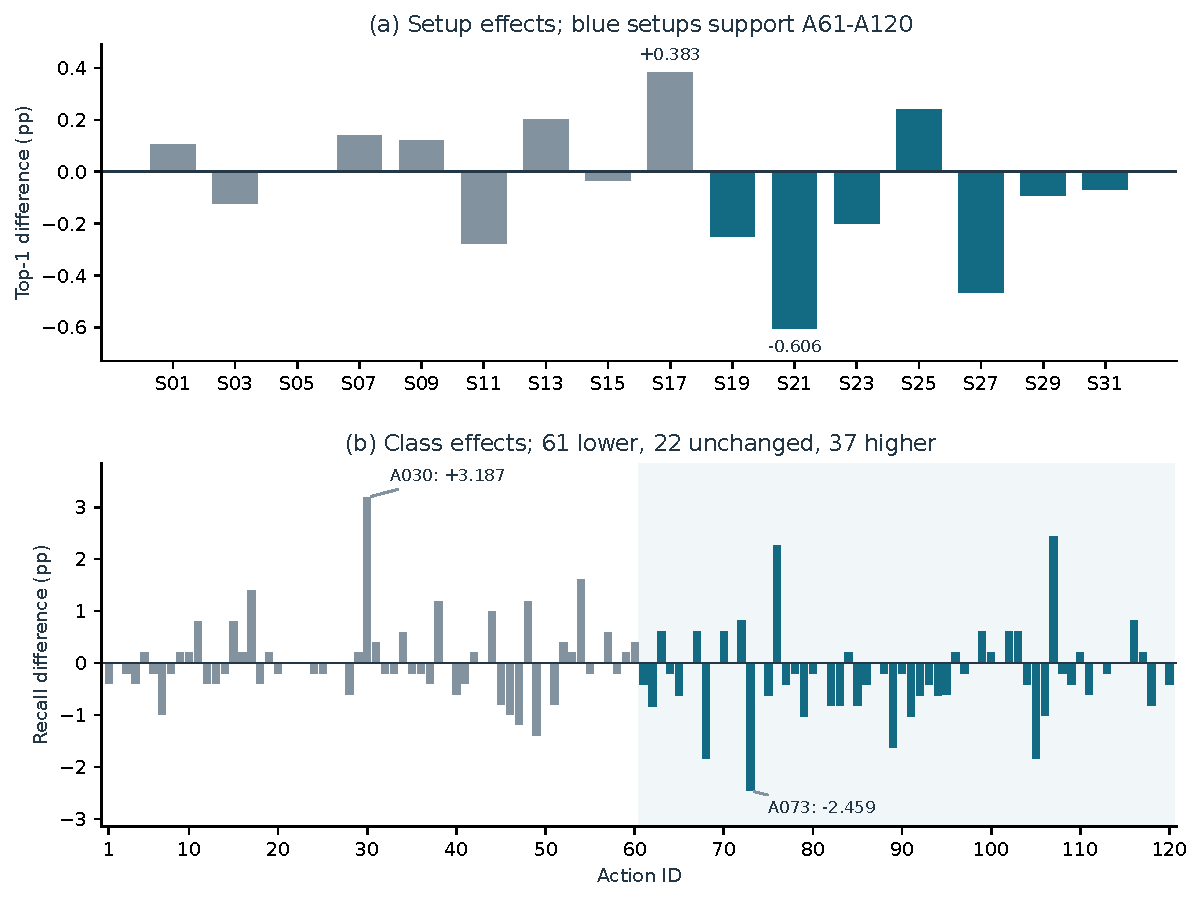
\includegraphics[width=0.97\linewidth]{figures/FINAL_HETEROGENEITY.pdf}
\caption{Descriptive final-test heterogeneity. Blue denotes the setups or
actions supporting A61--A120; gray denotes the earlier action group.
The two panels concern different metrics: Top-1 by setup and recall by
class. No additional inferential claim is drawn from these slices.}
\label{fig:heterogeneity}
\end{figure}


\FloatBarrier
\section{Discussion}

The two interventions act on different parts of the computation. Temporal reduction changes source access and the number of input positions, whereas removing a stream eliminates a complete network evaluation. In the recorded profile, inference latency changed little despite temporal reduction, and inference still accounted for most of the measured time. These observations account for the small end-to-end saving in this implementation; the profile does not isolate a hardware-level cause. Removing one sequential stream reduced latency by approximately one quarter. The same ordering need not hold when video decoding, pose estimation, or data transfer contributes substantially to total cost. Moreover, the temporal comparison changes both the number of observations and their resampling rule; it does not isolate a universal effect of frame count.

\subsection{Implications for Multi-Stream GNN Design}
The omitted bone-motion branch is not the weakest standalone classifier in the final evaluation: its Top-1 accuracy is 82.0183\%, compared with 81.4483\% for joints and 81.9695\% for joint motion. Standalone accuracy therefore does not determine a branch's marginal contribution to the ensemble. The paired results assess that contribution through changes in the decisions of the complete system. They support evaluating representations jointly with the retained branches and the fixed fusion rule, rather than ranking them only as separate classifiers.

The net accuracy difference corresponds to fewer than one additional error per 1,000 examples, but nearly 30 predicted labels per 1,000 examples changed. This distinction matters when errors have unequal consequences. The observed balance of corrected and introduced errors may be acceptable for one application and unacceptable for another, especially when an affected action is important. Aggregate non-inferiority and class-level descriptions answer different questions and should be reported together.

For a new application, the practical sequence is to profile the actual timing boundary, specify acceptable quality losses before evaluating the final candidate, and then inspect the paired error changes alongside aggregate metrics. Shared retained checkpoints make the comparison interpretable by avoiding an additional source of training variation between the two systems. Our experiment demonstrates this assessment for a single selected stream reduction; it does not show that the same branch should be removed from every multi-stream GNN.

Skeleton recognition is one component of action analysis in video streams. Reducing its cost may help when several cameras or sequences must share a computing budget. The present experiments use presegmented clips and provided skeleton coordinates. They do not measure pose estimation, action localization in continuous video, or operation on an embedded device. Evaluating these stages together is necessary before extending the findings to a complete video-analysis system.

\subsection{Limits of the Evidence}
The final Top-1 values are higher than the development values, but this
change cannot be attributed solely to a better operating point. The final
models use a larger training population and a different evaluation population.
Only the paired Full-4/Stream-3 comparison within each stage has the stated
controlled interpretation. Combining fold checkpoints into an additional
ensemble would also change the number of forwards and would define another
system; that option was not used.

The held-out evidence remains within NTU RGB+D 120. Earlier NTU60 work
limits the interpretation of A1--A60 as untouched by the project history.
A61--A120 is therefore the stronger held-out component, but it contains
samples from only seven setups. Even with 29,375 samples, the effective
cluster count for that endpoint remains small. Cluster-bootstrap inference
is approximate and conditional on these fitted models. It does not quantify
training variability over many independent seeds, subject-level dependence
across setups, or uncertainty on another dataset.

Non-inferiority is defined by the fixed margins. It does not imply equality, general
equivalence, or preservation of each action. The 61 decreases in class recall
and the worst-class decrease of 2.4590 percentage points are material limits
of an aggregate claim. An application that places special weight on an
affected action could reach a different practical assessment without changing
the scientific result of this prespecified comparison.

The latency evidence is restricted to one RTX 4090 environment, batch size
one, and the stated timing boundary. Final seed-161803 models were not timed
again. The historical latency campaign therefore supports the architecture
and stream-composition comparison on its own checkpoints, not an independently
remeasured latency for every final model. The study measures neither energy
nor batched throughput and provides no direct cross-device claim.

The numerical reproduction establishes the consistency of the supplied final evidence. It does not replay training or test inference. A matched comparison with efficient architectures, a broader seed study, and measurements on additional devices would be required to assess whether the observed operating point remains competitive outside this implementation. No superiority over EfficientGCN, HPI-GCN, or other published recognition systems is established.

\section{Conclusions}
The measured value of a skeleton representation depends on its contribution to the complete recognition system and on the part of the computation that it affects. In the evaluated CTR-GCN pipeline, temporal reduction lowered source-frame access but did not meet the required latency--quality trade-off. Removing the bone-motion stream from the K64 system reduced earlier measured batch-one latency by 24.30--24.94\%. The final fixed three-stream comparison then met all three prespecified aggregate non-inferiority criteria on NTU120 XSet, with 46 fewer correct predictions among 59,477 examples.

The small net loss combined 605 introduced and 559 corrected errors; a further 614 predictions changed between incorrect labels. These changes explain why aggregate quality tolerances must be interpreted together with class-level effects. The study provides a reproducible evaluation protocol and empirical guidance for this stream-reduction choice. Its extension to other backbones, independently trained systems, devices, and complete video pipelines remains to be tested. The final checkpoints were not included in a new latency measurement.

\supplementary{The supplementary document contains complete setup and action-class results, implementation details, and the scope of numerical reproduction. Exact CSV tables accompany the manuscript package.}
\authorcontributions{Conceptualization, A.I. and M.O.; methodology, O.K. and M.O.; software, O.K.; validation, A.S.; formal analysis, A.S.; investigation, L.Z.; resources, L.Z.; data curation, L.Z.; writing---original draft preparation, O.K.; visualization, A.N. and M.O.; supervision, A.N.; project administration, A.I.; funding acquisition, L.Z.}
\funding{This research has been funded by the Science Committee of the Ministry of Science and Higher Education of the Republic of Kazakhstan (Grant No. AP23486538 Research and development of a system for recognizing images in video streams based on artificial intelligence).}
\institutionalreview{This study is a secondary computational analysis of an existing action-recognition dataset; no new participants were recruited. No new intervention or data collection involving human participants was conducted.}
\informedconsent{No new participant data were collected. Access to the original NTU RGB+D 120 data follows the dataset provider's procedure.}
\dataavailability{The original NTU RGB+D 120 data are available through ROSE Lab, Nanyang Technological University \cite{ntuofficial}. The research package contains code, frozen protocols, trained checkpoints, saved predictions, and scripts for reproducing the reported analysis. The code and research artifact are available at \url{https://github.com/KuznetsovKarazin/aura-ksp}; versioned models and prediction files accompany its release. The original dataset is not redistributed.}
\acknowledgments{This research used the NTU RGB+D 120 Action Recognition Dataset provided by ROSE Lab, Nanyang Technological University, Singapore. ChatGPT (OpenAI) assisted with code and analysis development, interpretation, and manuscript preparation as described in the Materials and Methods. The authors are responsible for verifying the supporting code and evidence and for the submitted text.}
\conflictsofinterest{Author declarations and the role of the funder are to be confirmed before submission.}
\reftitle{References}
\bibliography{references}
\end{document}
